\documentclass[11pt]{article}
\usepackage[a4paper,margin=1in]{geometry}
\usepackage[T1]{fontenc}
\usepackage{lmodern}
\usepackage{microtype}
\usepackage{amsmath,amssymb,amsthm,mathtools}
\usepackage{enumitem}
\usepackage{booktabs}
\usepackage{tikz}
\usepackage{fancyhdr}
\PassOptionsToPackage{hyphens}{url}
\usepackage[hidelinks]{hyperref}

\setlength{\parskip}{0.5em}
\setlength{\parindent}{0pt}
\pagestyle{fancy}\fancyhf{}
\fancyhead[L]{\small The odd torus after $C_3 \mathbin{\square} C_n$}
\fancyhead[R]{\small\thepage}
\renewcommand{\headrulewidth}{0.4pt}

\theoremstyle{plain}
\newtheorem{theorem}{Theorem}[section]
\newtheorem{lemma}[theorem]{Lemma}
\newtheorem{corollary}[theorem]{Corollary}
\newtheorem{known}[theorem]{Known result}
\newtheorem{computed}[theorem]{Computer-assisted result}
\newtheorem{verified}[theorem]{Verified, not proved}
\newtheorem{openprob}[theorem]{Open problem}
\theoremstyle{definition}
\newtheorem{definition}[theorem]{Definition}
\newtheorem{fact}[theorem]{Fact}
\theoremstyle{remark}
\newtheorem{remark}[theorem]{Remark}

\newcommand{\T}{\mathbin{\square}}
\newcommand{\Z}{\mathbb{Z}}
\newcommand{\Q}{\mathbb{Q}}
\newcommand{\C}{\mathbb{C}}
\newcommand{\sm}{\setminus}
\newcommand{\script}[1]{\texttt{#1}}
\newenvironment{steps}[1][]{\begin{enumerate}[label=\textbf{Step \arabic*.},leftmargin=4.4em,itemsep=0.35em,#1]}{\end{enumerate}}

\title{List Colouring the Odd Torus:\\ Everything After $C_3 \T C_n$}
\author{Siddharth Narayan Mishra \and Amrutanshu}
\date{29 October 2026}

\begin{document}
\maketitle

\begin{abstract}
\noindent
This document starts where the proof that $C_3 \T C_n$ is 3-choosable ends. It collects every
result we have obtained since then on the conjecture of Cai, Wang and Zhu that every toroidal grid
$C_m \T C_n$ is 3-choosable, in the only open case where $m$ and $n$ are both odd. It gives full
proofs of everything proved by hand, states exactly what is established by computation and how, and
separates both from what is only supported by experiments. It ends with the precise list of problems
that still stand between us and the case $C_5 \T C_n$, and with the directions and ideas for the
general case.
\end{abstract}

\tableofcontents

%=====================================================================================
\section*{How to read this document}
\addcontentsline{toc}{section}{How to read this document}

Every numbered result carries one of these labels.

\begin{center}
\renewcommand{\arraystretch}{1.25}
\begin{tabular}{@{}p{5.2cm}p{9.6cm}@{}}
\toprule
\textbf{Known result} & published by others; cited, not proved here\\
\textbf{Theorem, Lemma, Corollary, Fact} & proved here by hand, every step written out\\
\textbf{Computer-assisted result} & proved, but one step is an exact finite computation (script named)\\
\textbf{Verified, not proved} & true in every case tested; no proof\\
\textbf{Open problem} & not known\\
\bottomrule
\end{tabular}
\end{center}

All script paths are relative to \script{\textasciitilde/work/gt/odd-torus/}. Appendix~\ref{app:scripts}
lists them together.

\textbf{Notation.}
\begin{itemize}[nosep]
\item $C_k$ is the cycle on $\Z_k$; $P_\ell$ is the path on $\{1, \dots, \ell\}$.
\item $C_m \T C_n$ has vertices $(i, j)$, $i \in \Z_m$ the \emph{row}, $j \in \Z_n$ the \emph{column}. The vertex
$(i,j)$ is adjacent to its \emph{column neighbours} $(i \pm 1, j)$ and its \emph{row neighbours} $(i, j \pm 1)$.
Each column induces $C_m$, each row induces $C_n$, and every vertex has degree 4.
\item A \emph{list assignment} $L$ gives each vertex a set $L(v)$; unless said otherwise $|L(v)| = 3$. An
\emph{$L$-colouring} is a proper colouring $c$ with $c(v) \in L(v)$ for all $v$. A list assignment with no
$L$-colouring is \emph{bad}.
\item The \emph{palette} is the union of all lists.
\item Throughout, ``odd torus'' means $C_m \T C_n$ with $m, n \ge 3$ both odd.
\end{itemize}

%=====================================================================================
\section{Starting point}\label{sec:start}

\subsection{What the talk establishes}

The talk before this document proves the following, and we use it freely.

\begin{theorem}[Theorem A]\label{thmA}
$C_3 \T C_n$ is 3-choosable for every $n \ge 3$.
\end{theorem}

Its proof uses three ingredients that we also reuse:
\begin{enumerate}[nosep]
\item the \emph{shape lemma} (Lemma~\ref{shape} below), which is how the Combinatorial Nullstellensatz is
used to \emph{pin} and \emph{forbid} colours;
\item the \emph{odd strip lemma} for $m = 3$: for odd $\ell \ge 3$, the strip $C_3 \T P_\ell$ with a pin on one
end column and a forbid on a different row of the other end column has coefficient $\pm 3^{(\ell-1)/2} \ne 0$;
\item the \emph{two-column (prism) lemma}, proved by exhaustive computation
(\script{ws-W9/prism\_sizes.c}), with a hand proof by Amrutanshu still to be merged.
\end{enumerate}

\subsection{Known results we use}

\begin{known}[Li, Shao, Petrov and Gordeev \cite{LSPG}]\label{lspg}
If $m$ or $n$ is even, $C_m \T C_n$ is 3-choosable. If $m$ and $n$ are both odd, the Alon--Tarsi number of
$C_m \T C_n$ is 4.
\end{known}

The second sentence is the reason the odd case is hard: the polynomial method applied to the whole torus
cannot prove 3-choosability, so every proof must at some point look at the actual lists.

\begin{known}[Combinatorial Nullstellensatz, Alon \cite{Alon}]\label{cn}
Let $P \in \C[x_1, \dots, x_N]$ have degree $\sum_i t_i$ with all $t_i \ge 0$, and suppose the coefficient of
$\prod_i x_i^{t_i}$ in $P$ is nonzero. If $S_1, \dots, S_N \subseteq \C$ satisfy $|S_i| > t_i$, then there is
$s \in S_1 \times \dots \times S_N$ with $P(s) \ne 0$.
\end{known}

\begin{known}[Erd\H{o}s, Rubin and Taylor \cite{ERT}]\label{cycle}
Let $C$ be a cycle and $|L(v)| \ge 2$ for every vertex of $C$. Then $C$ is $L$-colourable, unless $C$ is odd and all
the lists are the same set of size exactly 2.
\end{known}

\begin{known}[Alon and Tarsi \cite{AT}]\label{at}
Let $D$ be an orientation of a graph $G$. If the numbers of even and of odd Eulerian subgraphs of $D$ differ,
then $G$ is $L$-colourable whenever $|L(v)| > \mathrm{outdeg}_D(v)$ for every $v$.
\end{known}

\begin{known}[Hakimi \cite{Hak}]\label{hakimi}
Let $k : V(G) \to \Z_{\ge 0}$. A graph $G$ has an orientation with $\mathrm{outdeg}(v) \le k(v)$ for every $v$ if and
only if every subgraph $H$ satisfies $|E(H)| \le \sum_{v \in V(H)} k(v)$. It suffices to check induced subgraphs.
\end{known}

(The last sentence holds because adding edges to $H$ while keeping its vertex set only increases the left side.)

\subsection{Elementary facts, with proofs}

\begin{fact}[sum colourings]\label{sumcol}
Let $f : \Z_m \to \Z_3$ be a proper colouring of $C_m$ and $g : \Z_n \to \Z_3$ a proper colouring of $C_n$. Then
$\psi(i, j) = f(i) + g(j)$ is a proper colouring of $C_m \T C_n$ with values in $\Z_3$. Proper 3-colourings of
odd cycles exist, so every odd torus is 3-colourable.
\end{fact}

\begin{proof}
For a column edge $(i,j)(i+1,j)$: $\psi(i+1,j) - \psi(i,j) = f(i+1) - f(i) \ne 0$ because $f$ is proper. For a row
edge $(i,j)(i,j+1)$: $\psi(i,j+1) - \psi(i,j) = g(j+1) - g(j) \ne 0$ because $g$ is proper. A proper 3-colouring
of an odd cycle $C_k$ is $0, 1, 0, 1, \dots, 0, 1, 2$ (the last vertex is adjacent to the first, coloured $0$,
and to the one before it, coloured $1$).
\end{proof}

\begin{definition}[patterns]\label{pattern}
A \emph{column pattern} for column $j$ of $C_m \T C_n$ is a proper colouring $P$ of $C_m$ with $P_r \in L(r, j)$
for every row $r$. Two patterns $P, Q$ (of any columns) are \emph{compatible}, written $P \sim Q$, if $P_r \ne Q_r$
for every row $r$.
\end{definition}

\begin{fact}\label{patfact}
An $L$-colouring of $C_m \T C_n$ is the same thing as a choice of one pattern $P^{(j)}$ for each column $j$ such
that $P^{(j)} \sim P^{(j+1)}$ for every $j \in \Z_n$.
\end{fact}

\begin{proof}
The edges of the torus are the column edges, which lie inside one column, and the row edges
$(r, j)(r, j+1)$. A colouring is proper on the column edges of column $j$ exactly when its restriction to
column $j$ is a proper colouring of $C_m$; it lies in the lists exactly when that restriction is a pattern. It
is proper on the row edges between columns $j$ and $j+1$ exactly when the two restrictions differ in every row.
\end{proof}

\begin{definition}[spare room and shapes]\label{shapedef}
Fix an orientation of a graph $H$ with $N$ vertices and let $P_H = \prod_{(u,v)} (x_u - x_v)$, one factor per arc.
The \emph{spare room} of $H$ is $d(H) = 2N - |E(H)|$. A \emph{shape} is a map $\mu : V(H) \to \{0,1,2\}$ with
$\sum_v \mu(v) = d(H)$. Its \emph{coefficient} is $c_\mu = \big[\prod_v x_v^{2 - \mu(v)}\big] P_H$.
\end{definition}

Changing the orientation multiplies $P_H$ by $\pm 1$, so whether $c_\mu = 0$ does not depend on it.

\begin{lemma}[shape lemma]\label{shape}
Let $\mu$ be a shape for $H$ with $c_\mu \ne 0$. Let each vertex have a list $L(v)$ of 3 colours, and choose any
$L'(v) \subseteq L(v)$ with $|L'(v)| = 3 - \mu(v)$. Then $H$ has a proper colouring $c$ with $c(v) \in L'(v)$ for
every $v$.
\end{lemma}

\begin{proof}
\begin{steps}
\item Each factor $x_u - x_v$ is a nonzero homogeneous polynomial of degree 1. A product of nonzero
polynomials is nonzero, and a product of homogeneous polynomials is homogeneous with degree the sum of the
degrees. So $P_H$ is nonzero and homogeneous of degree $|E(H)|$.
\item Put $t_v = 2 - \mu(v) \ge 0$. Then $\sum_v t_v = 2N - \sum_v \mu(v) = 2N - d(H) = |E(H)| = \deg P_H$.
\item Map the colours injectively into $\C$. Then $L'(v)$ becomes $S_v \subseteq \C$ with
$|S_v| = 3 - \mu(v) = t_v + 1 > t_v$.
\item The coefficient of $\prod_v x_v^{t_v}$ in $P_H$ is $c_\mu \ne 0$, so Known result~\ref{cn} gives
$s \in \prod_v S_v$ with $P_H(s) \ne 0$.
\item $P_H(s) \ne 0$ means $s_u - s_v \ne 0$ for every arc, that is, for every edge. So $c(v) = s_v$ is a proper
colouring, and $c(v) \in L'(v)$. \qedhere
\end{steps}
\end{proof}

So spending one unit at $v$ ($\mu(v) = 1$) lets us \emph{forbid} any one colour $\beta \in L(v)$, by taking
$L'(v) = L(v) \sm \{\beta\}$; spending two units ($\mu(v) = 2$) lets us \emph{pin} $v$ to any $\alpha \in L(v)$, by
taking $L'(v) = \{\alpha\}$. The lemma promises \emph{some} colouring obeying these choices and nothing else, so
every argument that uses it has to work against \emph{every} such colouring.

\begin{corollary}[adjacent pins are useless]\label{adjpin}
If $\mu(u) = \mu(v) = 2$ for adjacent $u, v$, then $c_\mu = 0$.
\end{corollary}

\begin{proof}
Suppose $c_\mu \ne 0$. Give every vertex the list $\{1,2,3\}$ and take $L'(u) = L'(v) = \{1\}$. Lemma~\ref{shape}
gives a proper colouring with $c(u) = c(v) = 1$, which is impossible since $u$ and $v$ are adjacent.
\end{proof}

\begin{lemma}[counting the spare room]\label{spare}
Let $m, n \ge 3$ and $\ell \ge 2$.
\begin{enumerate}[label=(\alph*),nosep]
\item $C_m \T C_n$ has spare room $0$.
\item The strip $C_m \T P_\ell$ has spare room $m$.
\item For $n \ge 5$ and $m \ge 5$, removing a $3 \times 2$ block of vertices (three consecutive rows, two consecutive
columns) from $C_m \T C_n$ leaves a graph with spare room $5$.
\end{enumerate}
\end{lemma}

\begin{proof}
(a) $N = mn$ and every vertex has degree 4, so $|E| = 4N/2 = 2N$.

(b) $N = m\ell$. Each of the $\ell$ columns is a copy of $C_m$, giving $m\ell$ edges. Each of the $\ell - 1$ pairs of
consecutive columns is joined by $m$ row edges, giving $m(\ell - 1)$ edges. Total $2m\ell - m = 2N - m$.

(c) The six block vertices have degree sum $24$ in the torus. Inside the block there are $7$ edges: in each of the
two columns, two edges joining the three consecutive rows (the first and third rows of the block are not adjacent
because $m \ge 5$), and $3$ row edges between the two columns. Each of these is counted twice in the degree sum, so
$24 - 14 = 10$ edges leave the block. Removing the block removes $7 + 10 = 17$ edges. What is left has
$N' = mn - 6$ vertices and $2mn - 17 = 2(mn - 6) - 5 = 2N' - 5$ edges.
\end{proof}

%=====================================================================================
\section{Consequences of Theorem A for every odd torus}\label{sec:general}

In this section $m, n \ge 3$ are odd unless stated otherwise. Every result here is proved by hand and holds for
every palette.

\subsection{Constant rows or columns}

\begin{lemma}[three compatible columns]\label{xyz}
Let $a, b \ge 3$ be odd, and let $L$ be a list assignment of $C_a \T C_b$ with $L(i, j) = A_i$ for all $i, j$ (every
row has a constant list). Then $C_a \T C_b$ is $L$-colourable.
\end{lemma}

\begin{proof}
\begin{steps}
\item The map $(i, j) \mapsto (j, i)$ is an isomorphism $C_a \T C_3 \to C_3 \T C_a$. By Theorem~\ref{thmA} (with
$n = a$), $C_a \T C_3$ is 3-choosable. Give vertex $(i, j)$ of $C_a \T C_3$ the list $A_i$ and take an
$L$-colouring.
\item Let $X, Y, Z$ be its three columns. Each is a proper colouring of $C_a$ with $X_i, Y_i, Z_i \in A_i$, so each is
a pattern for every column of $C_a \T C_b$ (all columns have the same lists).
\item Row $i$ of $C_a \T C_3$ is a triangle, so $X_i, Y_i, Z_i$ are pairwise different. Hence $X \sim Y$, $Y \sim Z$,
$Z \sim X$.
\item Colour column $j$ of $C_a \T C_b$ by $X$ if $j = 0$, by $Y$ if $j$ is odd, and by $Z$ if $j \ge 2$ is even.
Since $b \ge 3$, columns $1$ and $2$ exist. Consecutive columns $(j, j+1)$ with $0 \le j \le b - 2$ get one of
$(X, Y)$, $(Y, Z)$, $(Z, Y)$. The last column $b - 1$ is even (as $b$ is odd) and $b - 1 \ge 2$, so it gets $Z$,
and the pair of columns $(b - 1, 0)$ gets $(Z, X)$. All these pairs are compatible, so by Fact~\ref{patfact} this
is an $L$-colouring. \qedhere
\end{steps}
\end{proof}

\begin{corollary}[row-constant or column-constant]\label{rowconst}
If $L$ is constant along every row, or constant along every column, then $C_m \T C_n$ is $L$-colourable.
\end{corollary}

\begin{proof}
Constant along every row: Lemma~\ref{xyz} with $(a, b) = (m, n)$. Constant along every column, $L(i,j) = B_j$: the
isomorphism $(i, j) \mapsto (j, i)$ from $C_m \T C_n$ to $C_n \T C_m$ turns this into an assignment of $C_n \T C_m$
that is constant along every row, and Lemma~\ref{xyz} with $(a, b) = (n, m)$ applies.
\end{proof}

\subsection{One free row}

\begin{lemma}[one free row]\label{freerow}
Let $m \ge 5$ and $n \ge 3$ be odd. Suppose there are a row $i_0$ and a 3-set $A$ with $L(i, j) = A$ for every
$i \ne i_0$ and every $j$. Then $C_m \T C_n$ is $L$-colourable.
\end{lemma}

\begin{proof}
\begin{steps}
\item \emph{The path of rows.} The rows other than $i_0$ are $i_0 + 1, i_0 + 2, \dots, i_0 + m - 1 = i_0 - 1$.
In $C_m$ they induce a path $R$ with $m - 1$ vertices, an even number at least $4$, whose ends are $i_0 + 1$ and
$i_0 - 1$. Since $m \ge 5$ these ends are not adjacent in $C_m$.
\item \emph{A colouring of $R$ with equal ends.} Let $p : R \to \Z_3$ take the values $0, 1, 2, 0$ on the first four
rows of $R$, followed by $1, 0, 1, 0, \dots, 1, 0$ on the remaining $m - 5$ rows (an even number). Consecutive values
differ, so $p$ is a proper colouring of the path $R$, and both ends get the value $0$.
\item \emph{Shifts along the columns.} We want $\sigma_0, \dots, \sigma_{n-1} \in \{+1, -1\}$ with
$\sum_j \sigma_j \equiv 0 \pmod 3$. If $k$ of them are $+1$, the sum is $k - (n - k) = 2k - n$. Choose
$k \in \{0, 1, 2\}$ with $2k \equiv n \pmod 3$ (possible because $2$ is invertible mod $3$); since $n \ge 3$, there
are enough indices. Put $t_0 = 0$ and $t_{j+1} = t_j + \sigma_j$ for $0 \le j \le n - 2$. Then
$t_0 - t_{n-1} = \sigma_{n-1}$ as well, because $\sum_j \sigma_j \equiv 0$. So for \emph{every} $j \in \Z_n$,
$t_{j+1} - t_j = \sigma_j \in \{\pm 1\}$, indices mod $n$.
\item \emph{Colouring the rows of $R$.} Fix a bijection $\pi : \Z_3 \to A$ and colour $(i, j)$, $i \in R$, with
$\pi(p(i) + t_j) \in A = L(i, j)$. Column edges inside $R$: $p(i) \ne p(i+1)$, so the values differ and $\pi$ is
injective. Row edges: $(p(i) + t_{j+1}) - (p(i) + t_j) = \sigma_j \ne 0$. So this is proper on every edge not meeting
row $i_0$.
\item \emph{What row $i_0$ sees.} The column neighbours of $(i_0, j)$ are $(i_0 \pm 1, j)$, the two ends of $R$, and both
are coloured $a_j := \pi(0 + t_j)$. Let $L'(i_0, j) = L(i_0, j) \sm \{a_j\}$, of size $\ge 2$. Row $i_0$ is a cycle $C_n$; a
colouring of it from the lists $L'$ completes an $L$-colouring of the torus, since its other neighbours are in row
$i_0$ itself.
\item \emph{When the cycle fails.} By Known result~\ref{cycle}, row $i_0$ can be coloured unless all $L'(i_0, j)$ are
one 2-set $B$. Assume that. Then $|L'(i_0,j)| = 2$ forces $a_j \in L(i_0, j)$, so $L(i_0, j) = B \cup \{a_j\}$ with
$a_j \notin B$. Also $a_j \in A$. Since $t_{j+1} \ne t_j$ and $\pi$ is injective, $a_{j+1} \ne a_j$, so the $a_j$ take at
least two distinct values, all in $A \sm B$. Hence $|A \sm B| \ge 2$.
\item \emph{A second try.} Let $\tau$ be a cyclic permutation of $A$ of order 3 (no fixed points) and replace $\pi$ by
$\tau \circ \pi$. Steps 4 and 5 still apply, with $a_j$ replaced by $\tau(a_j) \ne a_j$. Suppose row $i_0$ fails again.
By Step 6 applied again, $\tau(a_j) \in L(i_0, j) = B \cup \{a_j\}$, and $\tau(a_j) \ne a_j$, so $\tau(a_j) \in B$ for every
$j$. Then $\tau$ maps the at least two distinct values $a_j$ injectively into $A \cap B$, so $|A \cap B| \ge 2 = |B|$,
so $B \subseteq A$ and $|A \sm B| = 1$. This contradicts Step 6. So one of the two tries succeeds. \qedhere
\end{steps}
\end{proof}

\subsection{Merging colours}

\begin{lemma}[Lemma M, merging]\label{merge}
Let $G$ be any graph with a list assignment $L$, and suppose two colours $c \ne d$ never lie in a common list. Let
$\mathsf{m}$ be the map on colours that sends $d$ to $c$ and fixes everything else, and let $L'(v) = \mathsf{m}(L(v))$.
If $G$ is $L'$-colourable, then $G$ is $L$-colourable. Moreover $|L'(v)| = |L(v)|$.
\end{lemma}

\begin{proof}
\begin{steps}
\item $\mathsf{m}$ is injective on each $L(v)$: the only two colours it identifies are $c$ and $d$, which are never in
the same list. So $|L'(v)| = |L(v)|$, and for each $x \in L'(v)$ there is exactly one $y \in L(v)$ with
$\mathsf{m}(y) = x$.
\item Let $\varphi$ be an $L'$-colouring. Define $\psi(v)$ as the unique $y \in L(v)$ with $\mathsf{m}(y) = \varphi(v)$. Then
$\psi(v) \in L(v)$ and $\mathsf{m} \circ \psi = \varphi$.
\item If $u, v$ are adjacent and $\psi(u) = \psi(v)$, then $\varphi(u) = \mathsf{m}(\psi(u)) = \mathsf{m}(\psi(v)) = \varphi(v)$,
which is impossible. So $\psi$ is proper. \qedhere
\end{steps}
\end{proof}

\begin{corollary}[saturated counterexamples]\label{saturated}
If $C_m \T C_n$ has a bad 3-list assignment, it has one in which every two colours of the palette lie in a common
list. Such an assignment uses at most $k$ colours, where $\binom{k}{2} \le 3mn$. For $C_5 \T C_5$, $k \le 12$.
\end{corollary}

\begin{proof}
Start from a bad $L$. While two colours never share a list, merge them (Lemma~\ref{merge}). By the contrapositive
of Lemma~\ref{merge} the new assignment is still bad, its lists still have size 3, and the palette shrinks by one.
So the process stops, at a bad assignment in which every pair of colours shares a list. Each list contains
$\binom32 = 3$ pairs and there are $mn$ lists, so at most $3mn$ pairs are covered, and all $\binom{k}{2}$ pairs must be.
For $m = n = 5$: $\binom{12}{2} = 66 \le 75 < 78 = \binom{13}{2}$.
\end{proof}

\subsection{Projection and the sea lemma}

\begin{definition}[colour graph]
The \emph{colour graph} $K(L)$ has the colours of the palette as vertices, two colours being adjacent when they lie in a
common list. Each list induces a triangle in $K(L)$.
\end{definition}

\begin{lemma}[projection]\label{projection}
If $K(L)$ has a proper 3-colouring, then $C_m \T C_n$ is $L$-colourable.
\end{lemma}

\begin{proof}
Let $\pi$ be a proper colouring of $K(L)$ with values in $\Z_3$. On each list (a triangle of $K(L)$) $\pi$ takes three
different values, so it is a bijection $L(v) \to \Z_3$. Let $\psi$ be a proper colouring of the torus with values in
$\Z_3$ (Fact~\ref{sumcol}). Colour $v$ with the unique $c(v) \in L(v)$ with $\pi(c(v)) = \psi(v)$. If $u, v$ are
adjacent then $\psi(u) \ne \psi(v)$, so $\pi(c(u)) \ne \pi(c(v))$, so $c(u) \ne c(v)$.
\end{proof}

\begin{lemma}[sea lemma]\label{sea}
Let $X$ be a set of 3 colours. Call $v$ a \emph{defect} if $L(v) \ne X$, and put $O(v) = L(v) \sm X$, which is nonempty
for a defect (two different 3-sets). Suppose there is a set $T$ of defects such that
\begin{enumerate}[label=(\alph*),nosep]
\item the defects not in $T$ have a proper colouring using, at each such $v$, a colour of $O(v)$;
\item $T$ has at most one vertex in each column;
\item every $v \in T$ has $|O(v)| = 1$, so $L(v) \cap X = X \sm \{\phi_v\}$ for one colour $\phi_v \in X$;
\item it is not the case that $T$ meets every column, lies in a single row, and has all $\phi_v$ equal.
\end{enumerate}
Then $C_m \T C_n$ is $L$-colourable. The same holds with ``column'' and ``row'' exchanged in (b) and (d).
\end{lemma}

\begin{proof}
Identify $X$ with $\Z_3$. Fix a proper colouring $f$ of $C_m$ with values in $\Z_3$, to be adjusted in Step 6, and a
proper colouring $g$ of $C_n$, to be chosen in Step 4. Put $\psi(i, j) = f(i) + g(j)$, a proper colouring of the torus
(Fact~\ref{sumcol}).
\begin{steps}
\item \emph{The colouring.} Give a vertex with $L(v) = X$ the colour $\psi(v)$; give a defect not in $T$ its colour
from (a); give $v \in T$ the colour $\psi(v)$.
\item \emph{In the lists.} Non-defects: $\psi(v) \in \Z_3 = X = L(v)$. Defects not in $T$: by (a). For $v \in T$ we need
$\psi(v) \in L(v) \cap X = X \sm \{\phi_v\}$, that is, $\psi(v) \ne \phi_v$. This is ensured in Steps 4 to 6.
\item \emph{Proper.} Two vertices that both received a $\psi$-colour differ because $\psi$ is proper. Two defects not in
$T$ differ by (a). A defect not in $T$ has a colour outside $X$, and every other vertex has a colour in $X$, so they
differ.
\item \emph{The condition on $g$.} For $v = (i_v, j_v) \in T$, $\psi(v) \ne \phi_v$ means $g(j_v) \ne \phi_v - f(i_v)$. By (b)
each column $j$ has at most one $T$-vertex $v_j$. So $g$ must be a proper colouring of $C_n$ from the lists
$\Lambda_j = \Z_3 \sm \{h_j\}$ with $h_j = \phi_{v_j} - f(i_{v_j})$ if column $j$ meets $T$, and $\Lambda_j = \Z_3$
otherwise. All lists have size at least 2.
\item \emph{When $g$ fails.} By Known result~\ref{cycle} (here $n$ is odd), such $g$ exists unless every column meets $T$
and all $h_j$ are equal.
\item \emph{Two rows.} Suppose every column meets $T$ and $T$ meets two different rows $i_1 \ne i_2$, at columns
$j_1, j_2$. We show $f$ can be chosen with $h_{j_1} \ne h_{j_2}$, that is, $f(i_1) - f(i_2) \ne \phi_{v_{j_1}} - \phi_{v_{j_2}}
=: \delta$. First, there is a proper colouring $f$ of $C_m$ with $f(i_1) = 0$, $f(i_2) = 1$. Put these two values. The two
arcs of $C_m$ between $i_1$ and $i_2$ are paths. An arc with no inner vertex is the edge $i_1 i_2$, which is fine since
$0 \ne 1$. On an arc with inner vertices, colour them one by one starting next to $i_1$, each with a colour different from
the previous one; the last inner vertex has two coloured neighbours (the previous one, and $i_2$), so one of the three
colours is still free for it. Then $-f$ is also
proper, and the two give $f(i_1) - f(i_2) = -1$ and $= +1$. At least one of these differs from $\delta$.
\item \emph{One row.} If every column meets $T$ and $T$ lies in a single row $i_0$, then $h_j = \phi_{v_j} - f(i_0)$, and
these are all equal exactly when all $\phi_v$ are equal. Hypothesis (d) excludes this.
\item The version with rows and columns exchanged follows by the isomorphism $(i, j) \mapsto (j, i)$. \qedhere
\end{steps}
\end{proof}

\begin{remark}[generalised sea]\label{gensea}
Lemmas~\ref{projection} and~\ref{sea} combine. Replace ``$L(v) = X$'' by ``$L(v) \subseteq S$ and $\pi : S \to \Z_3$ is
one-to-one on $L(v)$'' for a fixed colour set $S$ and fixed map $\pi$, and let defects be the vertices whose list is not
inside $S$. The proof is the same, with $\psi(v)$ replaced by the colour of $L(v)$ that $\pi$ sends to $\psi(v)$. This is
the form used in Section~\ref{sec:hole}. The construction was also checked by machine on 3\,810 random seas
(\script{ws-W15/sea\_check.py}).
\end{remark}

\subsection{Seams with light overlap}

\begin{definition}[piecewise row-constant]\label{pwrc}
$L$ is \emph{piecewise row-constant} if the columns split, cyclically, into $k \ge 2$ consecutive blocks of at least
3 columns each, such that inside block $i$ row $r$ has a constant list $A^i_r$. The boundary between two blocks is a
\emph{seam}.
\end{definition}

\begin{lemma}[seam lemma, light overlap]\label{seamlight}
Let $m = 5$ and let $L$ be piecewise row-constant with $\sum_{r} |A^i_r \cap A^{i+1}_r| \le 8$ at every seam. Then
$C_5 \T C_n$ is $L$-colourable.
\end{lemma}

\begin{proof}
\begin{steps}
\item For each block $i$, colour $C_5 \T C_3$ from the row lists $A^i_r$ (Lemma~\ref{xyz}, Step 1). Its three columns
$X^i, Y^i, Z^i$ are patterns for every column of block $i$, pairwise compatible, and since row $r$ of $C_5 \T C_3$ is a
triangle, $\{X^i_r, Y^i_r, Z^i_r\} = A^i_r$.
\item \emph{One seam.} Consider the 9 pairs $(P, Q)$ with $P \in \{X^i, Y^i, Z^i\}$ and $Q \in \{X^{i+1}, Y^{i+1}, Z^{i+1}\}$.
The pair is incompatible exactly when $P_r = Q_r = c$ for some row $r$, and then $c \in A^i_r \cap A^{i+1}_r$. For each
row $r$ and each $c \in A^i_r \cap A^{i+1}_r$ there is exactly one $P$ with $P_r = c$ and exactly one $Q$ with $Q_r = c$,
by Step 1; so the pair $(r, c)$ spoils exactly one of the 9 pairs. There are at most 8 such pairs $(r, c)$, so at least one
of the 9 pairs is compatible. Fix one for every seam.
\item \emph{Walks on a triangle.} In the triangle on $\{X^i, Y^i, Z^i\}$, for every $s \ge 2$ and every two corners
$a, b$ there is a walk of exactly $s$ steps from $a$ to $b$. For $s = 2$: $a \to b' \to a$ with $b' \ne a$ if $b = a$, and
$a \to b'' \to b$ with $b''$ the third corner if $b \ne a$. If it holds for $s$, it holds for $s + 1$: to reach $b$, walk
$s$ steps to a corner $b' \ne b$ and step to $b$.
\item \emph{Inside a block.} Let block $i$ have $\ell \ge 3$ columns. Its first column must be the $Q$ chosen at its left
seam, and its last column the $P$ chosen at its right seam. By Step 3 with $s = \ell - 1 \ge 2$ there is a sequence of
columns from $Q$ to $P$ in which consecutive columns are different corners, hence compatible.
\item Every pair of consecutive columns is either inside a block (Step 4) or across a seam (Step 2), so Fact~\ref{patfact}
gives an $L$-colouring. \qedhere
\end{steps}
\end{proof}

This lemma is superseded by Corollary~\ref{pwrcind} below, which drops the overlap condition at the cost of an
induction on $n$. We keep it because it needs no induction hypothesis.

%=====================================================================================
\section{The triple-column reduction}\label{sec:triple}

From here until Section~\ref{sec:directions}, $m = 5$ and $n \ge 5$ is odd.

\begin{computed}[degenerate block; \script{ws-W17/degenerate\_fold.py}]\label{degen}
Let $E = \{e_1, e_2\}$ and let $x$ be a proper colouring of $C_5$ with no $x_r \in E$. Put $A_r = E \cup \{x_r\}$. Let $U, V$
be proper colourings of $C_5$ (with any colours) such that $U_r \ne x_r$ and $V_r \ne x_r$ for all $r$. Then there are
proper colourings $c^1, c^2, c^3$ of $C_5$ with $c^k_r \in A_r$ for all $r, k$, and $U \sim c^1 \sim c^2 \sim c^3 \sim V$.
\end{computed}

\begin{proof}
\begin{steps}
\item \emph{Only types matter.} For a pattern $c$ with $c_r \in A_r = \{e_1, e_2, x_r\}$, and since $U_r \ne x_r$, we have
$U_r = c_r$ only if $U_r \in E$ and $U_r = c_r$. So whether $U \sim c$ depends only on the \emph{type} vector of $U$: for
each $r$, whether $U_r = e_1$, $U_r = e_2$, or $U_r \notin A_r$ (``other''). The same holds for $V$.
\item \emph{Which types occur.} If $U$ is proper, then no two cyclically adjacent rows both have type $e_1$, or both have
type $e_2$. The check below covers every type vector with this property, which includes every type vector of a proper
$U$.
\item \emph{The finite check.} There are 81 proper colourings of $C_5$ from the lists $A_r$ and 81 admissible type
vectors. For each of the $81^2 = 6\,561$ pairs of type vectors for $(U, V)$ the script searches for $c^1, c^2, c^3$, and
finds them in every case (output: ``with no path: 0'', re-run on 29 October). \qedhere
\end{steps}
\end{proof}

\begin{theorem}[triple-column reduction]\label{triple}
Suppose $C_5 \T C_{n-2}$ is 3-choosable. If three consecutive columns $j, j+1, j+2$ of $C_5 \T C_n$ have identical lists,
$L(r, j) = L(r, j+1) = L(r, j+2) =: A_r$ for every $r$, then $C_5 \T C_n$ is $L$-colourable.
\end{theorem}

\begin{proof}
\begin{steps}
\item \emph{The smaller torus.} Delete columns $j+1$ and $j+2$ and join column $j$ to column $j+3$ by the row edges
$(r, j)(r, j+3)$. Since $n - 2 \ge 3$, the result is a copy of $C_5 \T C_{n-2}$, with columns
$j+3, j+4, \dots, j-1, j$ in cyclic order. Give it the inherited lists. By assumption it has an $L$-colouring
$\varphi$.
\item \emph{Patterns.} Let $P, U, V$ be the patterns of $\varphi$ on columns $j$, $j - 1$ and $j + 3$. In the smaller torus,
column $j$ is adjacent to columns $j - 1$ and $j + 3$, so $U \sim P$ and $P \sim V$.
\item \emph{What we need.} Keep $\varphi$ on all columns other than $j, j+1, j+2$. If we find patterns $c^1, c^2, c^3$ from the
lists $A_r$ with $U \sim c^1 \sim c^2 \sim c^3 \sim V$, then putting them on columns $j, j+1, j+2$ gives an $L$-colouring
of $C_5 \T C_n$ by Fact~\ref{patfact}: every other pair of consecutive columns is a pair of consecutive columns of the
smaller torus, coloured as before.
\item \emph{Case 1: the lists $A_r \sm \{P_r\}$ are not all the same 2-set.} Each has size 2, since $P_r \in A_r$. By Known
result~\ref{cycle} there is a proper colouring $W$ of $C_5$ with $W_r \in A_r \sm \{P_r\}$. Then $W \sim P$. Take
$c^1 = P$, $c^2 = W$, $c^3 = P$: $U \sim P \sim W \sim P \sim V$.
\item \emph{Case 2: $A_r \sm \{P_r\} = E$ for every $r$, for one 2-set $E$.} Then $A_r = E \cup \{P_r\}$ with $P_r \notin E$,
$P$ is a proper colouring of $C_5$, and $U_r \ne P_r$, $V_r \ne P_r$ by Step 2. This is exactly the hypothesis of
Result~\ref{degen} with $x = P$, which supplies $c^1, c^2, c^3$. \qedhere
\end{steps}
\end{proof}

\begin{corollary}[induction framework]\label{indframe}
To prove that $C_5 \T C_n$ is 3-choosable for every odd $n \ge 3$ it suffices to prove, for each odd $n \ge 5$ and
assuming $C_5 \T C_{n-2}$ is 3-choosable, that every 3-list assignment with no three identical consecutive columns
is colourable. The base case $n = 3$ is Theorem~\ref{thmA}, since $C_5 \T C_3 \cong C_3 \T C_5$.
\end{corollary}

\begin{corollary}[seams, any overlap]\label{pwrcind}
If $C_5 \T C_{n-2}$ is 3-choosable and $L$ is piecewise row-constant, then $C_5 \T C_n$ is $L$-colourable.
\end{corollary}

\begin{proof}
Every block has at least three columns, and inside a block every row is constant, so the first three columns of
any block are identical. Apply Theorem~\ref{triple}.
\end{proof}

%=====================================================================================
\section{Computer-assisted ingredients for $m = 5$}\label{sec:comp}

\subsection{How nonvanishing for all $n$ is proved}

Several results below say that a coefficient is nonzero for \emph{every} odd length. They all follow the same
argument, which we prove once.

\begin{lemma}[recurrence and dominance]\label{domroot}
Let $(s_j)_{j \ge 1}$ be a sequence of rational numbers that satisfies the linear recurrence with characteristic
polynomial $H = h_1 h_2$, where $h_1, h_2 \in \Q[y]$ are distinct monic irreducible polynomials all of whose roots are
negative real numbers, and $\deg H = d$. Then:
\begin{enumerate}[label=(\alph*),nosep]
\item the minimal polynomial $p$ of the sequence (the monic annihilating polynomial of least degree) is one of $1, h_1,
h_2, h_1 h_2$, and it can be read off exactly from $s_1, \dots, s_{2d}$;
\item if $p \ne 1$, write $s_j = \sum_{\rho} a_\rho \rho^j$ over the roots $\rho$ of $p$; then every $a_\rho \ne 0$;
\item if $p \ne 1$, let $\rho_1$ be the root of $p$ of largest modulus; it is unique, and if
$|a_{\rho_1}|\,|\rho_1|^{j_0} > \sum_{\rho \ne \rho_1} |a_\rho|\,|\rho|^{j_0}$, then $s_j \ne 0$ for every $j \ge j_0$.
\end{enumerate}
\end{lemma}

\begin{proof}
Let $\mathsf{E}$ be the shift, $(\mathsf{E}s)_j = s_{j+1}$. A polynomial $q$ \emph{annihilates} $s$ if $q(\mathsf{E})s = 0$.

(a) The annihilating polynomials over $\Q$ form an ideal of $\Q[y]$ containing $H$; its monic generator $p$ divides
$H = h_1 h_2$. Since $h_1, h_2$ are distinct and irreducible, $p \in \{1, h_1, h_2, h_1 h_2\}$. To decide whether a
divisor $q$ of $H$ annihilates $s$: the sequence $t = q(\mathsf{E}) s$ also satisfies the recurrence $H$, because
$H(\mathsf{E}) q(\mathsf{E}) s = q(\mathsf{E}) H(\mathsf{E}) s = 0$. A sequence satisfying a recurrence of order $d$ is zero if
its first $d$ terms are zero. The first $d$ terms of $t$ involve $s_1, \dots, s_{d + \deg q}$, and $\deg q \le d$.

(b) An irreducible polynomial over $\Q$ has distinct roots, and two distinct monic irreducibles have no common root,
so the roots of $H$ are distinct. Hence every sequence annihilated by $p$ has the form $\sum_\rho a_\rho \rho^j$ (standard
theory of linear recurrences with distinct roots). Suppose $a_{\rho'} = 0$ for some root $\rho'$. Then $s$ is
annihilated by $p / (y - \rho')$ over $\C$. But the minimal polynomial over $\C$ equals the one over $\Q$: ``there is a
monic annihilator of degree $e$'' is a system of linear equations in the unknown coefficients, with rational entries
(the $s_j$), and such a system has a complex solution if and only if it has a rational one (its solvability is decided
by ranks, which do not depend on the field). So the least degree is the same over $\Q$ and over $\C$, and the monic
annihilator of least degree is unique; it is $p$. This contradicts $\deg (p / (y - \rho')) < \deg p$.

(c) The roots are distinct negative reals, so their moduli are distinct, and the largest is attained once. Write
$s_j = a_{\rho_1}\rho_1^j\big(1 + \sum_{\rho \ne \rho_1} (a_\rho / a_{\rho_1}) (\rho / \rho_1)^j\big)$. The bracket is
nonzero when $\sum_{\rho \ne \rho_1} |a_\rho/a_{\rho_1}|\,|\rho/\rho_1|^j < 1$. Each term decreases in $j$ because
$|\rho/\rho_1| < 1$, so if this holds at $j_0$ it holds for all $j \ge j_0$; and it holding at $j_0$ is the stated
inequality. Since $a_{\rho_1} \ne 0$ by (b), $s_j \ne 0$ for $j \ge j_0$.
\end{proof}

In the applications the inequality in (c) is checked with certified interval (ball) arithmetic, and the finitely many
$j < j_0$ are computed exactly.

\subsection{The transfer matrix for $m = 5$}

For a strip or a torus with 5 rows, oriented $(r,c) \to (r+1,c)$ and $(r,c) \to (r,c+1)$, apply the coefficient formula
of Laso\'n and Karasev--Petrov \cite{Lason,KP} with every set equal to the cube roots of unity, exactly as in the strip
lemma for $m = 3$. The coefficient becomes a sum over all maps of the vertices to $\{1, \omega, \omega^2\}$ of the product
over arcs of $(x_u - x_v)$ times a monomial weight. Only proper colourings contribute, and a proper colouring of a column
$C_5$ with 3 colours is one of $2^5 - 2 = 30$ states. The sum therefore factorises along the columns as a product of
$30 \times 30$ matrices: the \emph{transfer matrix} $T$ (column arcs of the new column times row arcs to it), with
modified end matrices where weights are placed. Its relevant structural fact, computed exactly
(\script{ws-W4}), is:

\begin{computed}[\script{ws-W4}, item E2]\label{minpoly}
The minimal polynomial of $T$ is $x\, h_1(x^2)\, h_2(x^2)$ with
$h_1(y) = y^2 + 10y + 5$ and $h_2(y) = y^4 + 35y^3 + 110y^2 + 100y + 25$. Both are irreducible over $\Q$ and all their
roots are negative reals. The root of largest modulus gives the dominant pair of eigenvalues $\pm i\lambda_1$ of $T$,
$\lambda_1 \approx 5.6232$.
\end{computed}

(For $h_1$ the roots are $-5 \pm 2\sqrt5$, both negative. $h_2$ has positive coefficients, so no root is $\ge 0$; that
all its roots are real is part of the computation.) Hence for a sequence of the form $u^{\mathsf T} T^{2j+1} v$ (odd
lengths), the sequence $(s_j)_{j \ge 1}$ is annihilated by $h_1 h_2$ in $y = x^2$: indeed
$T \cdot h_1(T^2) h_2(T^2) = 0$ gives $T^{2} h_1(T^2) h_2(T^2) = 0$, so after one shift the factor $y$ drops. Lemma~\ref{domroot}
applies with $d = 6$.

\subsection{The results}

\begin{computed}[edge deletion; \script{ws-W4/}, see \script{ws-W4/REPORT.md}]\label{edgedel}
Let $m \in \{5, 7\}$ and $n \ge 3$ odd. For every edge $e$ of $G = C_m \T C_n$ and every vertex $w$ not on the column or row
cycle of $G$ through $e$, the coefficient of $x_w \prod_{v \ne w} x_v^2$ in $P_{G - e}$ is nonzero.
\end{computed}

Method: Lemma~\ref{domroot} with $T$ diagonalisable, a unique dominant pair, dominant amplitudes exactly nonzero, and the
leftover small $n$ computed exactly ($n_0 = 5$ for $m = 5$, $n_0 = 11$ for $m = 7$); exact values agree up to $n = 201$ with
an independent direct-expansion program.

\begin{corollary}\label{overlap}
For $m \in \{5, 7\}$, in every bad 3-list assignment of $C_m \T C_n$ ($n$ odd), every edge $uv$ has $L(u) \cap L(v) \ne \emptyset$.
\end{corollary}

\begin{proof}
Suppose $L(u) \cap L(v) = \emptyset$ for the edge $e = uv$. Choose $w$ off the cycle (column or row) containing $e$, and any 2-subset
$L'(w) \subseteq L(w)$. $G - e$ has $2N - 1$ edges, and the monomial $x_w \prod_{v \ne w} x_v^2$ has degree $2N - 1$, so by
Result~\ref{edgedel} and Known result~\ref{cn} (as in Lemma~\ref{shape}) $G - e$ has a proper colouring from the lists
$L'(w)$ and $L(v)$, $v \ne w$. It is also proper on $e$, because $u$ and $v$ receive colours from disjoint lists.
\end{proof}

\begin{computed}[odd strip lemma for $m = 5$; \script{ws-W7/prove\_strip5.py}]\label{strip5}
There are 74 shapes $\mu$ on $C_5 \T P_\ell$ that pin one vertex of one end column (weight 2), put weight 0 or 1 everywhere else
on the two end columns, and have $c_\mu \ne 0$ for every odd $\ell$ from 3 to 27. For each of them, in either orientation of
the strip, $c_\mu(\ell) \ne 0$ for \emph{every} odd $\ell \ge 3$.
\end{computed}

Method: $c_\mu(2j + 1) = u^{\mathsf T} T^{2j-1} v$; Lemma~\ref{domroot}. The minimal recurrence is $h_2$ in 96 and $h_1$ in 52 of
the 148 cases; the dominant term wins already at $j = 1$; the predicted recurrence was confirmed on exact values up to
$\ell = 41$.

\begin{remark}[midpoint rule]
For the shape ``pin at row $r$ of one end, forbid at the three rows of the other end outside $\{p, q\}$'', the coefficient
vanishes exactly when $\ell$ is odd and $2r \equiv p + q \pmod 5$ (checked for every $\ell$ from 2 to 27, 2\,600 cases,
\script{ws-W9/midpoint.py}). The zeros are forced: the row reflection fixing $r$ swaps $p$ and $q$, fixes the shape, and
reverses the $5\ell$ column arcs, an odd number when $\ell$ is odd, so it maps $c_\mu$ to $-c_\mu$.
\end{remark}

\begin{computed}[no small counterexample; \script{ws-W2/certify.py}]\label{c5c5}
There is no bad 3-list assignment of $C_5 \T C_5$ from a palette of 4 colours.
\end{computed}

Method: counterexample-guided search (an assignment proposed by a SAT solver is refuted by a colouring, which is turned
into a clause). The final master problem, without symmetry breaking, is unsatisfiable (97.7\,s); all 38\,400 cut clauses,
including their symmetry images, were re-verified independently, and an independent solver (glucose4) confirms
unsatisfiability. The 5-colour version stalls.

%=====================================================================================
\section{First route for $m = 5$: column cuts and windows}\label{sec:windows}

This route generalises the proof of Theorem~\ref{thmA} directly. It led to a theorem for 4 colours, and showed why a
second route was needed.

\subsection{The cut}

\begin{definition}[cut]\label{cutdef}
A \emph{trigger} is a pair $(r, j)$ with some $\alpha \in L(r, j) \sm L(r, j+1)$. The \emph{forward cut} at it deletes
columns $j+1$ and $j+2$; the rest is a strip $C_5 \T P_{n-2}$ with end columns $j+3$ and $j$, of odd length $n - 2 \ge 3$ and
spare room 5 (Lemma~\ref{spare}). We spend 2 units pinning $(r, j)$ to $\alpha$, and the other 3 on the two end columns as
allowed by one of the 74 shapes of Result~\ref{strip5}. A \emph{backward cut} is the mirror image (delete $j$ and $j - 1$,
using $\alpha' \in L(r, j+1) \sm L(r, j)$).
\end{definition}

After the strip is coloured, the two deleted columns form $C_5 \T K_2$, and each of its vertices loses at most the colour
of its one neighbour outside (in column $j$ or $j+3$). The pin makes sure $(r, j+1)$ loses nothing, since
$\alpha \notin L(r, j+1)$.

\begin{definition}[window]
A \emph{window} is the data that decides whether a cut can be completed: the 10 lists of the two deleted columns, and
$\alpha$. An \emph{adversary} chooses any proper colourings of the 5-cycles in columns $j$ and $j + 3$ (with $(r, j)$
coloured $\alpha$ and obeying the forbids). A window is \emph{good} if some shape and some choice of forbidden colours make
the fill of $C_5 \T K_2$ succeed against every adversary.
\end{definition}

\begin{theorem}[reduction for $m = 5$, first route]\label{red5}
Let $n \ge 5$ be odd. $C_5 \T C_n$ is $L$-colourable if $L$ is row-constant, column-constant, has one free row, or has a cut
whose window is good.
\end{theorem}

\begin{proof}
The first three cases are Corollary~\ref{rowconst} and Lemma~\ref{freerow}. For a good cut, the shape's coefficient is
nonzero at length $n - 2$ (Result~\ref{strip5}), so Lemma~\ref{shape} gives a colouring of the strip obeying the pin and the
forbids. Its restriction to columns $j$ and $j+3$ is one of the adversary's moves (the adversary may choose \emph{any}
proper colourings of those columns, so it is at least as strong as the real colouring). Goodness gives a colouring of the
two deleted columns compatible with it, and together they form an $L$-colouring.
\end{proof}

\subsection{What the computations showed}

\begin{computed}[palette of 4 colours; scripts in \script{ws-W8/}]\label{thmB}
Scripts: \script{window5.c}, \script{window5g.c}, \script{global\_q4\_all\_n.py}, \script{alln\_q4.py}.
\begin{enumerate}[label=(\alph*),nosep]
\item The single shape of the original plan is bad on 6\,904 of the $4^{10}$ windows; with all 74 shapes, 400 windows are
bad, and 184 once $\alpha$ is the actual colour.
\item For $n \in \{5, 7\}$, every 4-colour assignment in which every cut (forward and backward, at every trigger) is bad is
row-constant, column-constant, or has one free row (600 and 2\,520 assignments of the last kind).
\item \textbf{Theorem B.} For every odd $n$, $C_5 \T C_n$ is $L$-colourable whenever the palette has at most 4 colours.
``Every cut is bad'' becomes a closed walk in a finite graph of window states (262\,144 states); every part of that
graph carrying an odd closed walk consists of special assignments handled by Corollary~\ref{rowconst} or
Lemma~\ref{freerow}.
\end{enumerate}
\end{computed}

\begin{openprob}[window statement]\label{window}
Every 3-list assignment of $C_5 \T C_n$ ($n$ odd) in which every cut is bad is row-constant, column-constant, or has one free
row.
\end{openprob}

Together with Theorem~\ref{red5} this would prove the case $m = 5$. Evidence and dead ends:
\begin{itemize}[itemsep=0.2em]
\item With 5 and 6 colours there are new bad windows (992 within one changed list of a bad 4-colour window), but for
$n = 5$ the assignments built from them with every cut bad are again only column-constant (24) or one free row (39\,120).
\item No counterexample to Problem~\ref{window} was found by 16 hill-climbing runs (about 2 million steps, palettes 5 and 6).
\item ``Every bad window has at least 7 of its 10 lists equal to one 3-set'' is \textbf{false} (3 counterexamples with 6
equal lists, \script{ws-W11/hunt.c}). ``All lists within one colour of $X$, at least 3 rows equal to $X$'' is
\textbf{false} (1\,184 violations).
\item Verified, not proved: every bad window has 3 consecutive rows equal to one set in both columns (1\,395 bad windows, 9
unbiased hunts); every bad (window, $\alpha$) pair has at least 3 \emph{rigid} rows, $A_t = B_t$ (4\,731 pairs, 16 hunts
with 5 to 8 colours).
\item The fill of $C_5 \T K_2$ has no short list of failure patterns, unlike the prism for $m = 3$ (\script{ws-W10/prism5\_sample.py}).
Three-column cuts are much better on generic lists, but \emph{nearly constant} lists defeat every local cut
(\script{ws-W10/cut3\_nearconst.py}: 75 of 135 bad with one changed list).
\end{itemize}

\textbf{Conclusion of the first route.} A proof must split into a \emph{generic} regime, where a local cut works, and a
\emph{nearly constant} regime, where global constructions (Sections~\ref{sec:general} and~\ref{sec:triple}) are needed.
The hole route below is built around that split.

%=====================================================================================
\section{Second route for $m = 5$: the hole cut}\label{sec:hole}

\subsection{The hole}

Fix a row $t$ and a column $j$. The \emph{block} is the set of six vertices in rows $t - 1, t, t + 1$ and columns $j, j + 1$.
We name them $a_L, b_L, c_L$ (column $j$, rows $t-1, t, t+1$) and $a_R, b_R, c_R$ (column $j+1$). The \emph{border} is the
set of 10 vertices outside the block that have a neighbour in it:
\begin{center}
\begin{tabular}{@{}ll@{}}
$p_1, p_2, p_3$ & rows $t-1, t, t+1$ of column $j - 1$\\
$s_1, s_2, s_3$ & rows $t-1, t, t+1$ of column $j + 2$\\
$q_1, r_1$ & row $t + 2$, columns $j$ and $j + 1$\\
$q_2, r_2$ & row $t + 3 = t - 2$, columns $j$ and $j + 1$
\end{tabular}
\end{center}

\begin{center}
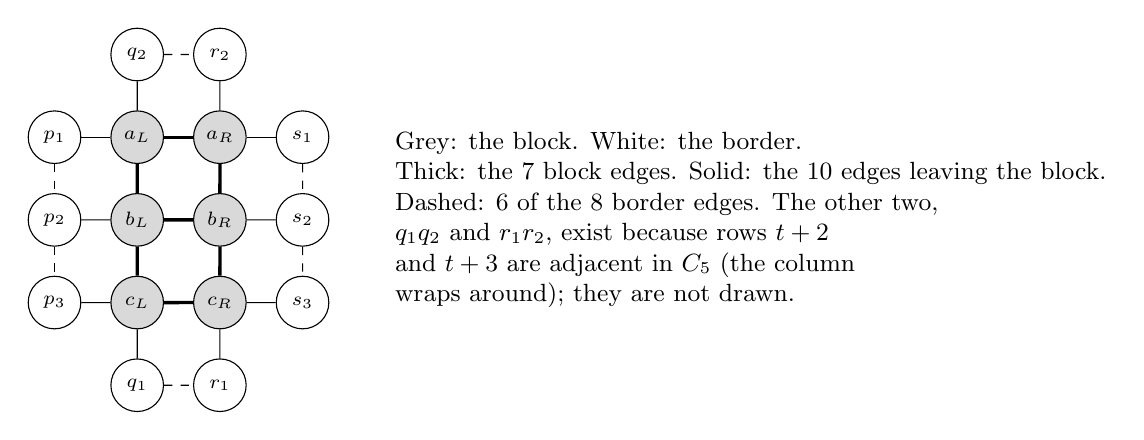
\begin{tikzpicture}[scale=1.05,v/.style={circle,draw,minimum size=19pt,inner sep=0pt,font=\scriptsize},
  blk/.style={v,fill=gray!30},brd/.style={v,fill=white}]
  \node[blk] (aL) at (1,0) {$a_L$}; \node[blk] (bL) at (1,-1) {$b_L$}; \node[blk] (cL) at (1,-2) {$c_L$};
  \node[blk] (aR) at (2,0) {$a_R$}; \node[blk] (bR) at (2,-1) {$b_R$}; \node[blk] (cR) at (2,-2) {$c_R$};
  \node[brd] (p1) at (0,0) {$p_1$}; \node[brd] (p2) at (0,-1) {$p_2$}; \node[brd] (p3) at (0,-2) {$p_3$};
  \node[brd] (s1) at (3,0) {$s_1$}; \node[brd] (s2) at (3,-1) {$s_2$}; \node[brd] (s3) at (3,-2) {$s_3$};
  \node[brd] (q2) at (1,1) {$q_2$}; \node[brd] (r2) at (2,1) {$r_2$};
  \node[brd] (q1) at (1,-3) {$q_1$}; \node[brd] (r1) at (2,-3) {$r_1$};
  \draw[very thick] (aL)--(bL)--(cL); \draw[very thick] (aR)--(bR)--(cR);
  \draw[very thick] (aL)--(aR); \draw[very thick] (bL)--(bR); \draw[very thick] (cL)--(cR);
  \draw (p1)--(aL); \draw (p2)--(bL); \draw (p3)--(cL); \draw (s1)--(aR); \draw (s2)--(bR); \draw (s3)--(cR);
  \draw (q2)--(aL); \draw (r2)--(aR); \draw (q1)--(cL); \draw (r1)--(cR);
  \draw[dashed] (p1)--(p2)--(p3); \draw[dashed] (s1)--(s2)--(s3); \draw[dashed] (q1)--(r1); \draw[dashed] (q2)--(r2);
  \node[font=\small,align=left,anchor=west] at (4,-1) {Grey: the block. White: the border.\\
  Thick: the 7 block edges. Solid: the 10 edges leaving the block.\\
  Dashed: 6 of the 8 border edges. The other two,\\ $q_1 q_2$ and $r_1 r_2$,
  exist because rows $t+2$\\ and $t+3$ are adjacent in $C_5$ (the column\\ wraps around); they are not drawn.};
\end{tikzpicture}
\end{center}

\begin{fact}\label{borderfact}
Let $m = 5$ and $n \ge 5$. The 10 edges leaving the block go to 10 distinct border vertices, each border vertex has exactly
one neighbour in the block, and the edges among border vertices are exactly the 8 edges $p_1p_2$, $p_2p_3$, $s_1s_2$,
$s_2s_3$, $q_1r_1$, $q_2r_2$, $q_1q_2$, $r_1r_2$.
\end{fact}

\begin{proof}
The block-to-outside edges are: $a_L p_1$, $b_L p_2$, $c_L p_3$ and $a_R s_1$, $b_R s_2$, $c_R s_3$ (row edges), and
$c_L q_1$, $a_L q_2$, $c_R r_1$, $a_R r_2$ (column edges: in column $j$ the rows next to the block are $t + 2$ below and
$t - 2 = t + 3$ above, and these are different rows of $C_5$). Columns $j - 1$ and $j + 2$ are different and outside the
block because $n \ge 4$. So the 10 endpoints are distinct, and each is adjacent to exactly one block vertex. Among them,
the $p$'s are three consecutive rows of one column (edges $p_1p_2$, $p_2p_3$; $p_1p_3$ is not an edge since $m = 5$), the
same for the $s$'s; $q_1, q_2$ are rows $t+2, t+3$ of column $j$, adjacent; $r_1, r_2$ likewise; $q_1 r_1$ and $q_2 r_2$ are
row edges. Vertices in columns $j-1$ and $j+2$ are not adjacent to vertices in columns $j, j+1$ of rows $t+2, t+3$ (different
rows and columns), and columns $j - 1, j + 2$ are not adjacent to each other when $n \ge 5$.
\end{proof}

The \emph{hole} is the block together with its border: 16 vertices and their 16 lists. Let $G'$ be the torus minus the
block. By Lemma~\ref{spare}(c) it has spare room 5, and since every vertex of $G'$ outside the border has all its neighbours
in $G'$, we spend the 5 units on the border.

\begin{computed}[hole coefficients; \script{ws-W14/hole\_coeff.py}, \script{hole\_prove.py}]\label{holecoef}
Of the 1\,388 ways of placing 5 units on the 10 border vertices (weights in $\{0,1,2\}$, no two adjacent border vertices both
pinned, as Corollary~\ref{adjpin} requires), exactly 1\,256 give a coefficient of $P_{G'}$ that is nonzero for \emph{every} odd
$n \ge 5$. Call this set of placements $\mathcal{M}$.
\end{computed}

Method: $c_\mu(n) = \mathrm{tr}(K T^{n-4})$ with the transfer matrix $T$ and a product $K$ of four modified column matrices,
computed exactly in $\Z[\omega]$; each of the two integer parts satisfies the recurrence of Result~\ref{minpoly}, and
Lemma~\ref{domroot} applies (19 exact terms). Sanity checks (\script{ws-W14/hole\_check.py}): on the full torus the same code gives
$\mathrm{tr}(T^n) = 0$ for odd $n$ and $\ne 0$ for even $n$, as Known result~\ref{lspg} predicts; and 1\,800 random list
assignments matching nonzero placements were all colourable.

\subsection{The hole game}

\begin{definition}[strategy, adversary, good hole]\label{game}
A \emph{strategy} for the hole is a placement $\mu \in \mathcal{M}$ together with a colour $\alpha_v \in L(v)$ for every
border vertex with $\mu(v) = 2$ and a colour $\beta_v \in L(v)$ for every border vertex with $\mu(v) = 1$. An
\emph{adversary move} is a choice $b_v \in L(v)$ for every border vertex $v$ with $b_v = \alpha_v$ where $\mu(v) = 2$ and
$b_v \ne \beta_v$ where $\mu(v) = 1$, which is proper on the 8 border edges. The strategy \emph{beats} the move if the block
has a proper colouring $f$ with $f(u) \in L(u) \sm \{b_w : w \text{ a border neighbour of } u\}$ for every block vertex $u$.
The hole is \emph{good} if some strategy beats every adversary move, and \emph{failing} otherwise. In the \emph{relaxed game}
the adversary need not be proper on the border edges; a hole good in the relaxed game is good.
\end{definition}

\begin{lemma}[hole reduction]\label{holered}
If some hole of $L$ is good, then $C_5 \T C_n$ is $L$-colourable.
\end{lemma}

\begin{proof}
\begin{steps}
\item Take a strategy that beats every move. Its placement $\mu$, extended by $0$ off the border, is a shape for $G'$
(the sum is $5 = d(G')$) with nonzero coefficient at this $n$ (Result~\ref{holecoef}).
\item Put $L'(v) = \{\alpha_v\}$ where $\mu(v) = 2$, $L'(v) = L(v) \sm \{\beta_v\}$ where $\mu(v) = 1$, and $L'(v) = L(v)$
otherwise. Lemma~\ref{shape} gives a proper colouring $c$ of $G'$ with $c(v) \in L'(v)$.
\item The restriction $b = c|_{\text{border}}$ is an adversary move: it lies in the lists, obeys the pins and forbids, and is
proper on the border edges because these are edges of $G'$.
\item The strategy beats $b$, so there is a block colouring $f$ as in Definition~\ref{game}.
\item Combine $c$ and $f$. Every edge of the torus lies in $G'$ (proper by Step 2), or in the block (proper by Step 4), or
joins a block vertex $u$ to a border vertex $w$ (Fact~\ref{borderfact}), where $f(u) \ne b_w = c(w)$ by Step 4. \qedhere
\end{steps}
\end{proof}

So only assignments in which \emph{every} one of the $5n$ holes fails remain.

\subsection{Filling the block}

\begin{lemma}[block-fill criterion]\label{blockfill}
After the border is coloured, let block vertex $u$ have lost $\ell_u$ colours, that is,
$\ell_u = |L(u) \cap \{b_w : w \text{ a border neighbour of } u\}|$. If for every set $S$ of block vertices
\[ \textstyle\sum_{u \in S} \ell_u \;\le\; 2|S| - e(S), \]
where $e(S)$ is the number of block edges with both ends in $S$, then the block can be filled.
\end{lemma}

\begin{proof}
\begin{steps}
\item Each block vertex has at most two border neighbours, so $\ell_u \le 2$; put $k(u) = 2 - \ell_u \ge 0$.
\item The condition says $e(S) \le \sum_{u \in S} k(u)$ for every $S$. By Known result~\ref{hakimi} the block has an
orientation $D$ with $\mathrm{outdeg}_D(u) \le k(u)$.
\item The remaining list of $u$ has size $3 - \ell_u = k(u) + 1 > \mathrm{outdeg}_D(u)$.
\item The block is the $3 \times 2$ grid, which is bipartite (colour a vertex by the parity of row plus column). In a bipartite
graph every cycle is even, and an Eulerian subgraph is an edge-disjoint union of cycles, so every Eulerian subgraph has an
even number of edges. Hence $D$ has no odd Eulerian subgraphs and at least one even one (the empty subgraph), so the counts
differ. Known result~\ref{at} fills the block. \qedhere
\end{steps}
\end{proof}

\subsection{Merging inside a hole}

\begin{lemma}[hole merging]\label{holemerge}
Suppose colours $c \ne d$ never lie in a common one of the 16 lists of a hole, and let $L'$ be obtained by replacing $d$ by
$c$ in these 16 lists. If the hole with lists $L'$ is good in the relaxed game, then the hole with lists $L$ is good in the
relaxed game. Consequently, every hole that fails in the relaxed game can be merged, step by step, into one that fails in
the relaxed game and uses at most 10 colours.
\end{lemma}

\begin{proof}
Let $\mathsf{m}$ send $d$ to $c$; it is injective on each of the 16 lists (as in Lemma~\ref{merge}, Step 1), so every $x \in
L'(v)$ has a unique preimage $\bar{x}^v \in L(v)$.
\begin{steps}
\item \emph{Transfer the strategy.} Let $(\mu, \alpha', \beta')$ be good for $L'$. Use the same $\mu$, with
$\alpha_v = \overline{\alpha'_v}^v$ and $\beta_v = \overline{\beta'_v}^v$.
\item \emph{Transfer the move.} Let $b$ be a relaxed move against it. Then $b' = \mathsf{m} \circ b$ is a relaxed move for $L'$:
$b'_v \in L'(v)$; at a pin $b'_v = \mathsf{m}(\alpha_v) = \alpha'_v$; at a forbid $b_v \ne \beta_v$ with both in $L(v)$, and
$\mathsf{m}$ is injective on $L(v)$, so $b'_v \ne \mathsf{m}(\beta_v) = \beta'_v$. (Properness on border edges is not needed;
it could fail, since $b_u = c$, $b_w = d$ becomes $b'_u = b'_w$. This is why the lemma is stated for the relaxed game.)
\item \emph{Transfer the fill.} The strategy for $L'$ beats $b'$: there is a block colouring $f'$ with $f'(u) \in L'(u)$ and
$f'(u) \ne b'_w$ for border neighbours $w$. Put $f(u) = \overline{f'(u)}^u$. Block edges: $f(u) = f(u_2)$ would give
$f'(u) = f'(u_2)$. Border edges $uw$: $f(u) = b_w$ would give $f'(u) = \mathsf{m}(f(u)) = \mathsf{m}(b_w) = b'_w$. So $f$ beats $b$.
\item \emph{The bound.} Repeat merging while two colours never share one of the 16 lists. By the contrapositive of Steps 1
to 3, failure in the relaxed game is preserved, and the palette shrinks each time. At the end every pair of colours shares
one of the 16 lists, which cover at most $16 \cdot 3 = 48$ pairs, so $\binom{k}{2} \le 48$ and $k \le 10$. \qedhere
\end{steps}
\end{proof}

\begin{computed}[isolated block; \script{ws-W14/block\_types\_allowed.c}]\label{isoblock}
If all six block lists of some hole equal one 3-set $X$ and all ten border lists differ from $X$, then that hole is good
(every odd $n \ge 5$, every palette). Hence $C_5 \T C_n$ is $L$-colourable.
\end{computed}

\begin{proof}
\begin{steps}
\item A border list $L(w) \ne X$ of size 3 contains at least one colour outside $X$, and $|L(w) \cap X| \le 2$.
\item For the fill, a border colour outside $X$ removes nothing from a block list (all block lists are $X$). So all colours
of $L(w) \sm X$ act the same, and only the \emph{type} $L(w) \cap X$ (a subset of $X$ of size at most 2: 7 types) matters,
together with one symbol ``outside''.
\item The program checks all $7^{10}$ type assignments of the border. For each it searches strategies with placements in
$\mathcal{M}$ (pin to a colour of the type or to ``outside'', forbid a colour of the type) against the relaxed adversary,
and finds a winning strategy every time. Since the relaxed game is harder for us, the hole is good, and
Lemma~\ref{holered} applies. \qedhere
\end{steps}
\end{proof}

\subsection{Failing holes: seas and seams}

\begin{definition}[local sea, local seam]\label{localdef}
Inside a hole, rows $t-1, t, t+1$ contain four hole vertices (columns $j - 1$ to $j + 2$) and rows $t + 2, t + 3$ contain two
(columns $j, j+1$).
\begin{itemize}[nosep]
\item The hole is a \emph{local seam} if there is a column boundary $\gamma \in \{\text{none}, (j{-}1 \mid j), (j \mid j{+}1),
(j{+}1 \mid j{+}2)\}$ such that in every row, hole vertices on the same side of $\gamma$ have equal lists.
\item The hole is a \emph{local sea} if its 16 lists satisfy the hypotheses of the generalised sea lemma
(Remark~\ref{gensea}) read inside the hole.
\end{itemize}
\end{definition}

\begin{verified}[\script{ws-W14/i2\_test.py}]\label{I2}
\textbf{(I$''$)} Every failing hole is a local sea or a local seam. Tested on 646 failing holes: 119 sea only, 98 seam only,
429 both, 0 neither. The sea-only failing holes have from 2 to 4 defects with respect to their majority set $X$ (119 of 119).
\end{verified}

\textbf{Caution.} These failing holes were found with the \emph{proper} adversary (Definition~\ref{game}). Lemma~\ref{holemerge}
is about the relaxed game. To use merging in a proof of (I$''$), either (I$''$) must be proved for holes failing in the relaxed
game (a larger class), or merging must be shown to work for the proper game. Moreover, ``local sea or seam'' does not
automatically survive un-merging (two lists $\{c, a, b\}$ and $\{d, a, b\}$ become equal after merging $d$ into $c$), so
reducing (I$''$) to holes with at most 10 colours needs an extra argument.

\subsection{Gluing seams}

Write $F(j)$ for the statement ``$L(r, j) = L(r, j+1)$ for every row $r$'' (the boundary $j \mid j+1$ is invisible).

\begin{theorem}[seam gluing]\label{seamglue}
Let $n \ge 5$ be odd. If every hole $(t, j)$, $t \in \Z_5$, $j \in \Z_n$, of $C_5 \T C_n$ is a local seam, then three consecutive
columns of $C_5 \T C_n$ have identical lists.
\end{theorem}

\begin{proof}
\begin{steps}
\item \emph{What each seam type gives.} Fix a hole $(t, j)$ and let $W = \{t-1, t, t+1\}$.
\begin{itemize}[nosep]
\item $\gamma$ = none, $(j{-}1 \mid j)$ or $(j{+}1 \mid j{+}2)$: in each of these, columns $j$ and $j+1$ are on the same side of
$\gamma$, so $L(r, j) = L(r, j+1)$ for all $r \in W$, and also for $r \in \{t+2, t+3\}$ (whose hole vertices are exactly columns
$j, j+1$). These are all 5 rows, so $F(j)$ holds.
\item $\gamma = (j \mid j{+}1)$: columns $j-1, j$ are on one side and $j+1, j+2$ on the other, so
$L(r, j-1) = L(r, j)$ and $L(r, j+1) = L(r, j+2)$ for every $r \in W$.
\end{itemize}
\item \emph{One column boundary.} Fix $j$ with $F(j)$ false. By Step 1 no hole $(t, j)$ has $\gamma \ne (j \mid j{+}1)$, so for
every $t \in \Z_5$ the rows $t - 1, t, t + 1$ satisfy $L(r, j-1) = L(r, j)$ and $L(r, j+1) = L(r, j+2)$. Every row $r$ lies in some
$\{t-1, t, t+1\}$ (take $t = r$). Hence $F(j - 1)$ and $F(j + 1)$ are both true.
\item \emph{Parity.} Suppose no $j$ has $F(j)$ and $F(j+1)$ both true. Then the set $\mathcal{F} = \{j : F(j)\}$ contains no two
cyclically consecutive elements of $\Z_n$. By Step 2, every $j \notin \mathcal{F}$ has $j - 1, j + 1 \in \mathcal{F}$, so the
complement contains no two consecutive elements either. Then colouring $j$ by whether $j \in \mathcal{F}$ is a proper
2-colouring of the cycle $C_n$, which is impossible because $n$ is odd.
\item So there is $j$ with $F(j)$ and $F(j+1)$, that is, columns $j, j+1, j+2$ are identical. \qedhere
\end{steps}
\end{proof}

\begin{corollary}[the all-seam case]\label{allseam}
If $C_5 \T C_{n-2}$ is 3-choosable and every hole of $L$ is a local seam, then $C_5 \T C_n$ is $L$-colourable.
\end{corollary}

\begin{proof}
Theorem~\ref{seamglue} and Theorem~\ref{triple}.
\end{proof}

\subsection{Gluing seas: what is known}

The remaining case is: every hole fails, no three consecutive columns are identical, and (assuming (I$''$)) every hole is a
local sea or a local seam, with at least one hole not a seam (otherwise Corollary~\ref{allseam} applies). The plan was to show
that all the local seas share one majority set $X$ and that the hypotheses of the sea lemma then hold globally.

\textbf{New finding (29 October).} The first half, in the abstract form we wrote down, is \textbf{false}. The script
\script{ws-W18/g1\_sat.py} encodes it as a SAT problem on abstract labels (equal labels mean equal lists): premises (i) no three
consecutive identical columns, (ii) every hole is a local seam or has at most 4 of its 16 vertices off one label $X$; negated
conclusion: for every label $X$ some hole has at least 5 vertices off $X$. For $n = 5$ and 3 labels it is satisfiable, for
example (rows top to bottom, columns left to right)
\[
\begin{matrix} 0&0&0&0&0\\ 1&1&0&0&0\\ 0&0&2&2&0\\ 0&0&0&0&0\\ 0&0&1&0&0 \end{matrix}
\]
Here label $0$ is the obvious sea, but some hole contains 5 non-$0$ vertices and is allowed only because it is a local seam.
So ``every hole is a sea with the same $X$'' cannot be the target: holes that are seams must be allowed to contain many
defects. This does not say that such an assignment is bad; the labels carry no list information. It says the gluing statement
must be reformulated, for example as ``the defects with respect to a single global $X$ satisfy the hypotheses of the sea lemma''
directly.

\subsection{Where $C_5 \T C_n$ stands}

\begin{theorem}[conditional result for $m = 5$]\label{conditional}
Suppose the following two statements hold for every odd $n \ge 5$.
\begin{enumerate}[label=(\Roman*),nosep]
\item Every failing hole of $C_5 \T C_n$ is a local sea or a local seam.
\item (Sea gluing.) If every hole fails, every hole is a local sea or a local seam, at least one hole is not a local seam, and
no three consecutive columns are identical, then $L$ satisfies the hypotheses of the generalised sea lemma
(Remark~\ref{gensea}), possibly with rows and columns exchanged, or is row-constant, column-constant or has one free row.
\end{enumerate}
Then $C_5 \T C_n$ is 3-choosable for every odd $n$, and so $\chi_\ell(C_5 \T C_n) = 3$ for every $n \ge 3$.
\end{theorem}

\begin{proof}
Induction on odd $n$. For $n = 3$: Theorem~\ref{thmA} with $C_5 \T C_3 \cong C_3 \T C_5$. Let $n \ge 5$, assume $C_5 \T C_{n-2}$ is
3-choosable, and let $L$ be any 3-list assignment of $C_5 \T C_n$.
\begin{enumerate}[label=(\arabic*),nosep]
\item If some hole is good: Lemma~\ref{holered}.
\item If three consecutive columns are identical: Theorem~\ref{triple}.
\item Otherwise every hole fails, so by (I) every hole is a local sea or a local seam. If all are local seams,
Theorem~\ref{seamglue} gives three identical consecutive columns, which is case (2). Otherwise (II) applies and
Lemma~\ref{sea} with Remark~\ref{gensea}, Corollary~\ref{rowconst} or Lemma~\ref{freerow} colours the torus.
\end{enumerate}
For even $n$, 3-choosability is Known result~\ref{lspg}. The lower bound $\chi_\ell \ge 3$ holds because every column is
an odd cycle, which is not 2-colourable.
\end{proof}

%=====================================================================================
\section{What must be solved for $C_5 \T C_n$}\label{sec:todo}

Everything in Theorem~\ref{conditional} is proved except (I) and (II). In order of how we plan to attack them:

\begin{openprob}[(II), sea gluing]\label{op2}
Prove statement (II) of Theorem~\ref{conditional}, in a corrected form.
\end{openprob}
\begin{itemize}[itemsep=0.2em]
\item \emph{First fix the statement.} The SAT counterexample of the previous section shows the local-count form is false.
Rerun \script{ws-W18/g1\_sat.py} with the conclusion replaced by the global sea hypotheses (defects w.r.t.\ one $X$; at most
one $T$-vertex per column; the exception (d)), and with labels replaced by actual lists from small palettes, so that the
answer is about real list assignments.
\item \emph{Then prove it.} Neighbouring holes share most of their vertices (holes $(t, j)$ and $(t, j+1)$ share 10), and a
sea-only failing hole has at most 4 defects; so two overlapping sea holes have the same majority set, and the set $X$ propagates
along chains of sea holes. Every column lies in one hole, so ``at most one $T$-vertex per column'' is a local condition.
The difficulty is where chains of seas pass through seam holes; the parity argument of Theorem~\ref{seamglue} is the
model for how such regions must close up around an odd cycle.
\end{itemize}

\begin{openprob}[(I), failing holes]\label{op1}
Prove that every failing hole is a local sea or a local seam, for every palette.
\end{openprob}
\begin{itemize}[itemsep=0.2em]
\item Settle the caution after Result~\ref{I2} first: decide whether to prove (I) for the relaxed game (then hole merging
applies, but the class is larger and (I) might fail) or to prove a version of merging for the proper game.
\item Case analysis by how much each border list shares with its block neighbour's list: if it shares one colour, one forbid
neutralises it; two colours, a pin to its third colour neutralises it; three colours (equal lists) it cannot be
neutralised. Equal lists across many of the 10 block-border edges is exactly ``nearly constant'', so the cases that survive
should be the seas and seams. Lemma~\ref{blockfill} turns each fill into counting losses.
\item The hole game for at most 10 colours is finite. A complete enumeration up to symmetry, of the kind used for
Result~\ref{isoblock}, would make (I) a computer-assisted result if the un-merging problem is solved.
\end{itemize}

\begin{openprob}[hand proofs of finite steps]\label{op3}
Give hand proofs of Result~\ref{degen} (degenerate block) and of the prism lemma for $m = 3$. Neither is needed for
correctness, but both are needed for a readable paper, and a hand proof of Result~\ref{degen} is what generalises to every
odd $m$ (Section~\ref{sec:directions}).
\end{openprob}

\textbf{Alternative if (I) and (II) resist.} Problem~\ref{window} (the window statement) is an independent route to the same
theorem; Theorem B shows it works for 4 colours. Evidence also points at a structural lemma for bad windows (at least 3
rigid rows) that may be easier than the full statement.

\textbf{Before submission of Theorem A.} Merge Amrutanshu's hand proof of the prism lemma; complete the literature check of
the papers citing \cite{LSPG} and of the dynamic survey, to make sure the odd case of $C_3 \T C_n$ is not already settled.

%=====================================================================================
\section{Directions for the general case $C_m \T C_n$, $m, n$ odd}\label{sec:directions}

\subsection{What already holds for every odd $m$}

Corollary~\ref{rowconst}, Lemmas~\ref{freerow}, \ref{merge}, \ref{projection}, \ref{sea}, Corollary~\ref{saturated} and the
counting Lemma~\ref{spare}(a), (b) hold for all odd $m, n$, with the same proofs. The hole has spare room 5 for every $m \ge 5$
(Lemma~\ref{spare}(c)), and Fact~\ref{borderfact}, Lemmas~\ref{holered}, \ref{blockfill} and \ref{holemerge} hold for every
$m \ge 5$ with the same proofs (the border rows $t + 2$ and $t - 2$ are distinct from the block rows and from each other; for
$m \ge 7$ they are no longer adjacent, so $q_1 q_2$ and $r_1 r_2$ stop being border edges, and the set of admissible
placements changes). The seam gluing argument (Theorem~\ref{seamglue}) does \emph{not} carry over directly: for $m = 5$ a
hole sees all 5 rows in columns $j, j+1$, which is what gives $F(j)$ in Step 1, while for $m \ge 7$ it sees only 5 of the
$m$ rows. A version for larger $m$ needs larger holes or an argument combining several holes in one column.

\subsection{What is specific to $m = 5$}

\begin{itemize}[itemsep=0.2em]
\item The transfer matrix: $2^m - 2$ states (30 for $m = 5$, 126 for $m = 7$). Edge deletion is already done for $m = 7$
(Result~\ref{edgedel}), so the strip and hole coefficients for $m = 7$ are within reach by the same method.
\item The degenerate block lemma (Result~\ref{degen}) was checked only for the 5-cycle.
\end{itemize}

\subsection{Ideas}

\begin{enumerate}[itemsep=0.35em]
\item \textbf{Double induction on $(m, n)$.} Theorem~\ref{triple} reduces $n$ by 2 when three columns are identical. Its transpose
reduces $m$ by 2 when three \emph{rows} are identical, provided the degenerate block lemma holds for the cycle $C_n$. So the key
lemma is:

\begin{openprob}[degenerate lemma for every odd cycle]\label{degenk}
For every odd $k \ge 3$: let $E = \{e_1, e_2\}$, $x$ a proper colouring of $C_k$ avoiding $E$, $A_r = E \cup \{x_r\}$, and $U, V$
proper colourings of $C_k$ with $U_r \ne x_r \ne V_r$. Then there are patterns $c^1, c^2, c^3$ from the $A_r$ with
$U \sim c^1 \sim c^2 \sim c^3 \sim V$.
\end{openprob}

Only types matter (Result~\ref{degen}, Step 1), so for each $k$ this is a finite check; a hand proof would come from a transfer
argument along the cycle. Note that $c^2 = x$ is never possible, since $c^1$ would then need values in $E$ only, a 2-colouring of
an odd cycle; so the three patterns must each use some of the $x_r$.

\item \textbf{A strip lemma uniform in $m$.} For $m = 3$ the strip coefficient has a closed form, $\pm 3^{(\ell-1)/2}$, from the
cube-root-of-unity evaluation. For $m = 5$ the eigenvalues come from $h_1(y) = y^2 + 10y + 5$, whose roots $-5 \pm 2\sqrt5$ lie in
$\Q(\sqrt5) \subset \Q(\zeta_5)$. This suggests that the spectrum of the transfer matrix for $C_m$ is governed by $\Q(\zeta_m)$ and
that a closed form, or at least a uniform dominance argument, exists for all $m$. (Speculative: not checked beyond $m = 5, 7$.)

\item \textbf{Nearly constant versus generic.} Every route so far splits into a generic regime handled by a local cut and a
nearly constant regime handled by global constructions (sum colourings, Theorem~\ref{triple}, Lemma~\ref{freerow}). A general
proof should make this split explicit: define a distance from a list assignment to the ``constant-like'' family (row-constant,
column-constant, sea, piecewise row-constant), and prove a local cut works above some threshold.

\item \textbf{Folding rows.} If rows $i - 1$ and $i + 1$ have equal lists in every column, identify them: this folds $C_m \T C_n$ to
$C_{m-2} \T C_n$ plus a free row. For $m = 5$ it reduces to $C_3 \T C_n$ with one list of size 2 (``Lemma S''), which was
confirmed exhaustively for $C_3 \T C_3$ with 4 colours (393\,216 assignments) and on 80\,000 random cases for $n = 5, 7$. A
proof of Lemma S would extend Theorem A and supply another reduction.

\item \textbf{Paintability.} The kernel method gives 3-paintability of $C_3 \T C_{3k}$ for odd $k$ (Amrutanshu), but our proof
of Theorem A does not, because $\beta$ is chosen from the lists in advance. Is $C_3 \T C_n$ 3-paintable for every odd $n$? The
kernel method is limited: for $n = 5, 7, 11, 13$ no orientation of $C_3 \T C_n$ with all out-degrees 2 is kernel-perfect.

\item \textbf{Computation as a guide.} Push the certified search to $C_5 \T C_5$ with 5 colours and to $C_5 \T C_7$ with
4 colours; and by Corollary~\ref{saturated} only saturated assignments (at most 12 colours for $C_5 \T C_5$) need to be searched.
\end{enumerate}

%=====================================================================================
\section{Other results from the same project}\label{sec:other}

These are not on the path to the torus theorem, but they were obtained in the same period. Proofs are in the files named.

\begin{itemize}[itemsep=0.3em]
\item \textbf{Kernel orientations of $C_3 \T C_n$} (\script{ws-W5}). The orientation $\varphi(i,j) = (i + j) \bmod 3$, column edges
towards the smaller colour, row edges towards the larger, is kernel-perfect on $C_3 \T C_{3k}$ exactly when
$k \not\equiv 2 \pmod 4$ (for $k \equiv 2 \pmod 4$ it contains an induced directed cycle of odd length $3n/2$). This corrects the
earlier claim that it fails for all even $k$. All old orientation counts were reproduced by independent code.
\item \textbf{2-d kernels in tori} (\script{ws-W3/REPORT.md}). $C_m \T C_n$ has a 2-d kernel (independent, and every outside
vertex has at least two out-arcs into it) if and only if $\gcd(m, n) > 1$; all of them are diagonal, and their number is
$2P(d) - 2[d \text{ even}]$ with $P$ the Perrin sequence and $d = \gcd(m,n)$. This contradicts Theorem 2.5 and Corollary 2.6
of Bednarz and W{\l}och (2016); for example $C_3 \T C_6$ has 6. In three dimensions, $C_3 \T C_b \T C_c$ has one if and only if
$3 \mid b$ or $3 \mid c$.
\item \textbf{Galvin's method on regular graphs} (\script{latex/galvin-converse-regular.tex}). For a $k$-regular graph $G$, $L(G)$
has a kernel-perfect orientation with all out-degrees at most $k - 1$ if and only if $G$ is bipartite.
\end{itemize}

%=====================================================================================
\appendix
\section{Where every computation lives}\label{app:scripts}

\begin{center}\small
\renewcommand{\arraystretch}{1.2}
\begin{tabular}{@{}p{4.3cm}p{5.6cm}p{4.6cm}@{}}
\toprule
Result & Script (in \script{odd-torus/}) & Output\\
\midrule
\ref{degen} degenerate block & \script{ws-W17/degenerate\_fold.py} & 0 of 6\,561 pairs without path\\
\ref{minpoly} minimal polynomial & \script{ws-W4/} & see \script{REPORT.md}\\
\ref{edgedel} edge deletion & \script{ws-W4/} & $n_0 = 5$ ($m=5$), $n_0 = 11$ ($m=7$)\\
\ref{strip5} strip, $m = 5$ & \script{ws-W7/prove\_strip5.py} & 148 cases proved\\
Midpoint rule & \script{ws-W9/midpoint.py} & 0 mismatches in 2\,600\\
\ref{c5c5} $C_5 \T C_5$, 4 colours & \script{ws-W2/certify.py} & UNSAT, certified\\
\ref{thmB} windows, Theorem B & \script{ws-W8/window5.c}, \script{window5g.c}, \script{alln\_q4.py} & 6\,904; 400; 184\\
Window evidence & \script{ws-W10/}, \script{ws-W11/} & see text\\
\ref{holecoef} hole coefficients & \script{ws-W14/hole\_coeff.py}, \script{hole\_prove.py}, \script{hole\_check.py} & 1\,256 placements\\
\ref{isoblock} isolated block & \script{ws-W14/block\_types\_allowed.c} & 0 type vectors without strategy\\
\ref{gensea} sea construction & \script{ws-W15/sea\_check.py} & 3\,810 of 3\,810\\
\ref{I2} (I$''$) & \script{ws-W14/i2\_test.py}, \script{sea\_profile.py} & 0 neither (646 holes)\\
Sea gluing, abstract form & \script{ws-W18/g1\_sat.py 5 3} & SAT: counterexample\\
Heavy seams (superseded) & \script{ws-W16/seam\_test.py} & 0 failures in 390\\
\bottomrule
\end{tabular}
\end{center}

\begin{thebibliography}{LSPG}
\bibitem[Alon]{Alon} N.~Alon, Combinatorial Nullstellensatz, \emph{Combin. Probab. Comput.} 8 (1999), 7--29.
\bibitem[AT]{AT} N.~Alon and M.~Tarsi, Colorings and orientations of graphs, \emph{Combinatorica} 12 (1992), 125--134.
\bibitem[CWZ]{CWZ} L.~Cai, W.~Wang and X.~Zhu, Choosability of toroidal graphs without short cycles, \emph{J. Graph
Theory} 65 (2010), 1--15.
\bibitem[ERT]{ERT} P.~Erd\H{o}s, A.~L.~Rubin and H.~Taylor, Choosability in graphs, \emph{Congr. Numer.} 26 (1979),
125--157.
\bibitem[Hak]{Hak} S.~L.~Hakimi, On the degrees of the vertices of a directed graph, \emph{J. Franklin Inst.} 279 (1965),
290--308.
\bibitem[KP]{KP} R.~N.~Karasev and F.~V.~Petrov, Partitions of nonzero elements of a finite field into pairs,
\emph{Israel J. Math.} 192 (2012), 143--156.
\bibitem[Lason]{Lason} M.~Laso\'n, A generalization of Combinatorial Nullstellensatz, \emph{Electron. J. Combin.} 17
(2010), \#N32.
\bibitem[LSPG]{LSPG} Z.~Li, Z.~Shao, F.~Petrov and A.~Gordeev, The Alon--Tarsi number of a toroidal grid,
\emph{European J. Combin.} 111 (2023), 103697.
\end{thebibliography}

\end{document}
